%%%%%%%%%%%%%%%%%%%%%%%%%%%%%%%%%%%%%%%%%
%
% (c) 2019 by Jennifer Laaser
%
% This work is licensed under the Creative Commons Attribution-NonCommercial-ShareAlike 4.0 International License. To view a copy of this license, visit http://creativecommons.org/licenses/by-nc-sa/4.0/ or send a letter to Creative Commons, PO Box 1866, Mountain View, CA 94042, USA.
%
% The current source for these materials is accessible on Github: https://github.com/jlaaser/pogil-polymers
%
%%%%%%%%%%%%%%%%%%%%%%%%%%%%%%%%%%%%%%%%%

\renewcommand{\figpath}{content/polymphys/solution-thermo/phase-diagrams/figs}
\renewcommand{\labelbase}{phase-diagrams}

\begin{activity}[Phase Diagrams of Polymer Solutions]

\begin{instructornotes}

	This activity introduces students to key concepts related to phase diagrams of polymer solutions.
	
	After completing this activity, students will be able to:
			\begin{enumerate}
				\item ...
			\end{enumerate}
	This activity will prepare students for ...
			
	\subsection*{Activity summary:}
	\begin{itemize}
		\item \textbf{Activity type:} Learning Cycle
		\item \textbf{Content goals:} Phase diagrams of polymer solutions
		\item \textbf{Process goals:} %https://pogil.org/uploads/attachments/cj54b5yts006cklx4hh758htf-process-skills-official-pogil-list-2015-original.pdf
			written communication, critical thinking, information processing
		\item \textbf{Duration:} TBD
		\item \textbf{Instructor preparation required:} none beyond knowledge of relevant content
		\item \textbf{Related textbook chapters:}
			\begin{itemize}
				\item \emph{Polymer Chemistry} (Hiemenz \& Lodge): sections XX \& YY
			\end{itemize}
	\end{itemize}

\end{instructornotes}

	%\textbf{Focus question:} Put a central question for the students to consider through this exercise here.


\begin{model}
\label{\labelbase:mdl:spinodalbinodal}

	Representative free energy curves for solutions of polymers with the same degree of polymerization, $N$, but different values of $\chi$, are shown below:
	
	\centerline{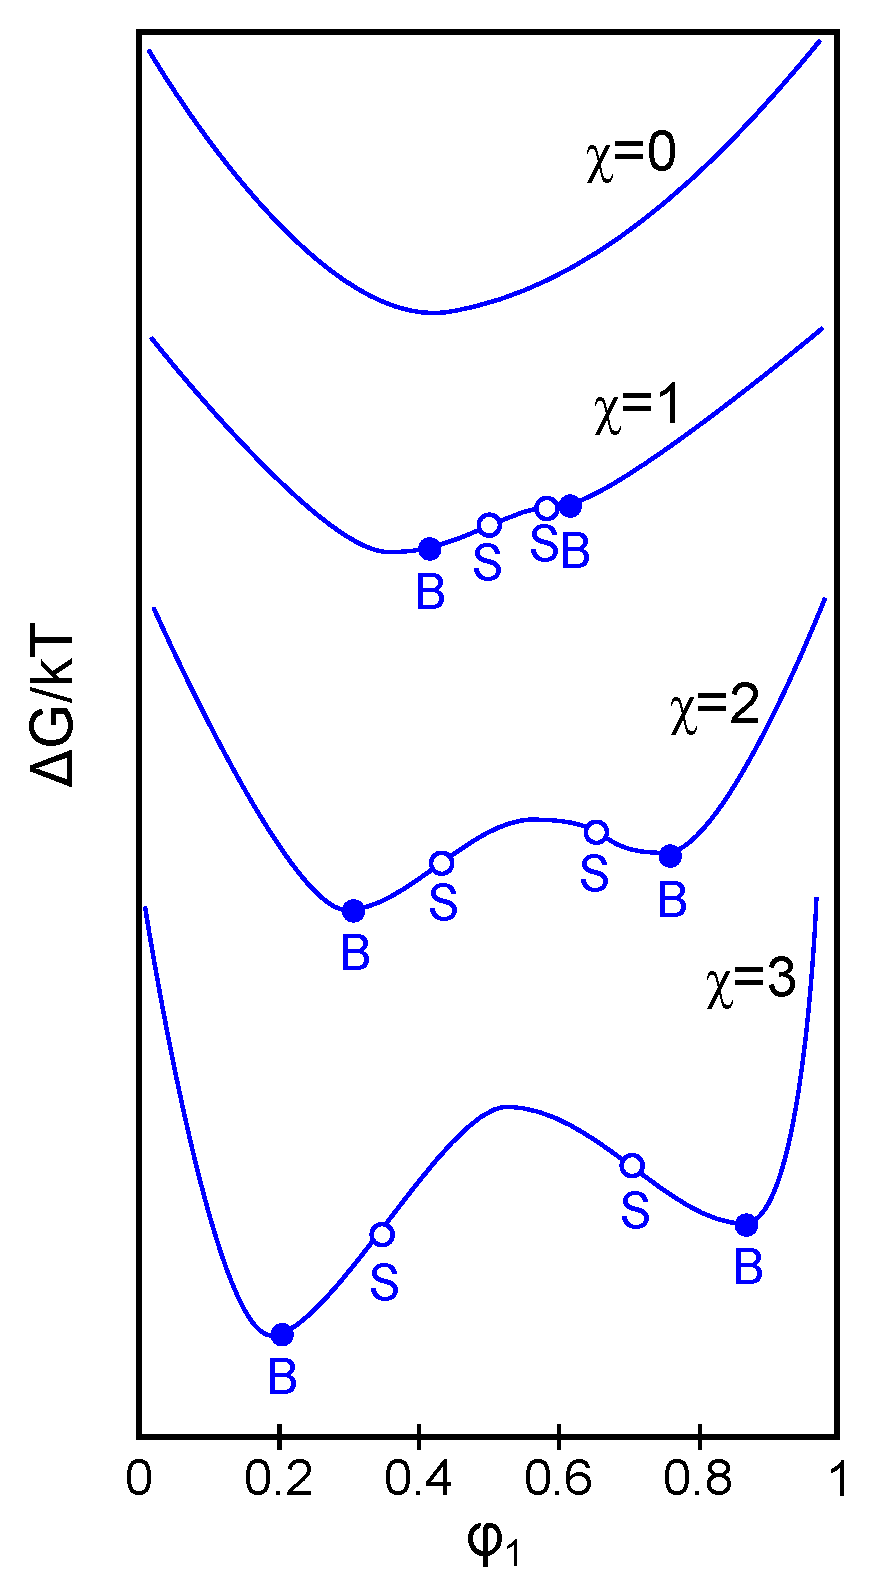
\includegraphics[width=0.4\textwidth]{\figpath/model1-varychi}}
	
	The spinodal (S) and binodal (B) points are marked on the plots where appropriate.
\end{model}

\begin{ctqs}
	
	\question Why doesn't the top plot ($\chi=0$) have any points marked on it?
	
	\question What do you think would happen to the positions of the spinodal and binodal points around $\chi=1/2$? Explain your reasoning in 1-2 complete sentences.
	
	\question Plot the locations of the spinodal and binodal points for each value of $\chi$ on the following axes.  When you have plotted all of the points, draw a smooth curve connecting all of the binodal points, and a second curve connecting all of the spinodal points.
	
		\centerline{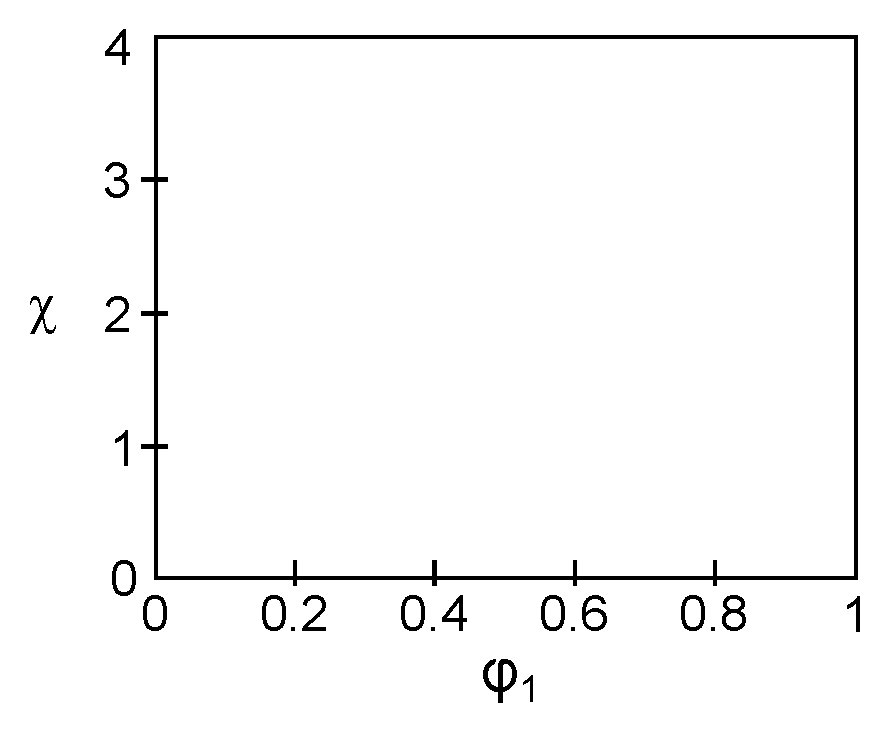
\includegraphics[width=0.4\textwidth]{\figpath/model1-phasediagramchi}}
		
\end{ctqs}


\begin{infobox}
	For a given polymer/solvent pair, the interaction parameter, $\chi$, generally varies with temperature as
	\begin{equation*}
		\chi \sim \frac{1}{T}
	\end{equation*}
\end{infobox}


\begin{ctqs}

	\question Re-plot your curves from the previous question with temperature on the y axis.
	
		\emph{Note: for the purposes of this question, assume that $\chi = \frac{100}{T}$.}
	
		\centerline{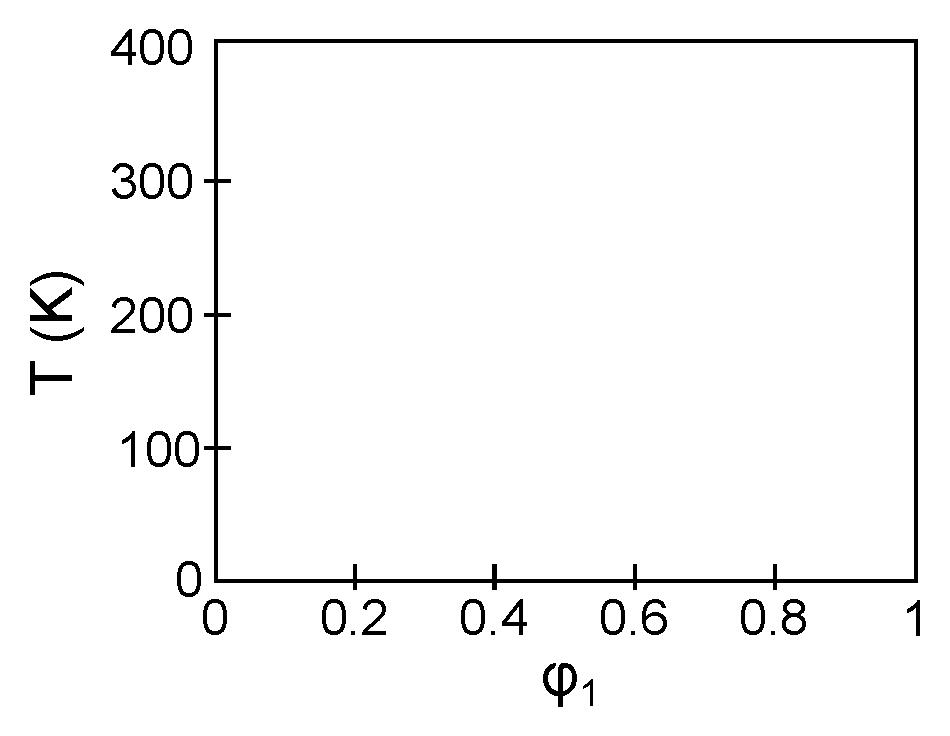
\includegraphics[width=0.4\textwidth]{\figpath/model1-phasediagramT}}
		
	\question Thinking back to the previous activity, how would you expect this diagram to change if you increased $N$, the degree of polymerization of the polymer?
		
\end{ctqs}



\begin{exercises}

		\exercise In Model 1, we  noted that there is some value of $\chi$ at which all of the phase boundaries (spinodal and binodal points) converge. This point is called the critical point of the polymer solution.
		
		Mathematically, how could you find the value of $\chi$ at which the critical point occurs?
		
		\emph{Hint: the spinodal points occur where $\frac{d^2\Delta G}{d\phi_1^2} = 0$.  What must happen to the \emph{third} derivative of $\Delta G$ when the spinodal points are in exactly the same place?}
		
		\exercise What do you expect would happen if you prepared a polymer solution at a very high temperature and then rapidly decreased the temperature of the mixture?
		
\end{exercises}
	
\end{activity}